\clearpage

\appendix

\section{Model implementation details} \label{sec:model_details}

All models are implemented using the Huggingface Transformers package \cite{Wolf2019HuggingFacesTS}.

%%%%%%%%%%%%%%%%%%%%

\subsection{Parameters for the final \sysname system} \label{sec:parameters}

For the \componentone module, \sysname retrieves the top $k=3$ documents ranked by TF-IDF similarity using unigram + bigram features. These parameters are tuned on the \ours development set.

When making predictions using the \componenttwo module described in \S\ref{sec:rationale_selection}, we find that the usual decision rule of predicting $\hat{z}_i = 1$ when $\tilde{z}_i \geq 0.5$ works well for models trained on \ours. However, for models trained on \fever and \snopes, we achieve better performance by tuning the classification threshold $t$, such that $\hat{z}_i = 1$  when $\tilde{z}_i \geq t$, on the \ours dev set. The best threshold was $t=0.025$ when training on \fever, and $t=0.75$ when training on \snopes.


%%%%%%%%%%%%%%%%%%%%


\subsection{Training the \componenttwo module}

We experiment with various learning rates when training \scibert, \bioroberta, \robertabase, and \robertalarge. Below we describe the setting for training \robertalarge.

For models trained on \ours, we use an initial learning rate of 1e-5 on the transformer base and 1e-3 on the linear layer. For \fever + \ours, the learning rate is set to 1e-5 for the entire model for pre-training on \fever and fine-tuning on \ours. We use a batch size of 256 through gradient accumulation and apply cosine learning rate decay over 20 epochs to find the best performing model on the dev set.

For models trained on \fever, we set the learning rate to 5e-6 for the transformer base and 5e-5 for the linear layer. For models trained on \snopes, we set the learning rate 1e-5 for the transformer base and 1e-4 for the linear layer. We find that these learning rates help the models converge. We only train the model for 3 epochs on \fever and 5 epochs on \snopes because they are larger datasets and the models converged within early epochs.

%%%%%%%%%%%%%%%%%%%%

\subsection{Training the \componentthree module}

We adopt similar settings as we used for the \componenttwo module and only change the learning rate to 1e-5 for the transformer base and 1e-4 for the linear layer for models trained on \ours, \fever, and \snopes. When training on claim / cited abstract pairs labeled \notenough, we use the $k$ sentences in the abstract with greatest similarity to the claim as rationales (\S\ref{sec:baselines}). $k$ is sampled from $\{0, 1\}$ with uniform probability.

%%%%%%%%%%%%%%%%%%%%


\subsection{Additional Training details}

All models are trained using a single Nvidia P100 GPU on Google Colabortoary Pro platform.\footnote{\url{https://colab.research.google.com/}} For the \componenttwo module, it takes about 150 minutes to train on \ours for 20 epochs. 120 minutes on \snopes for 5 epochs, and 700 minutes on \fever for 3 epochs. For the \componentthree module, it takes about 130 minutes to train on \ours for 20 epochs, 160 minutes on \snopes for 5 epochs, and 640 minutes on \fever for 3 epochs.

%%%%%%%%%%%%%%%%%%%%


\subsection{Hyperparameters search}

The learning rate, batch size, and number of epochs are the most important hyperparameters. We perform manual tuning and select the hyperparameters that produce the highest F1 on the development set. For the learning rate, we experiment with 1e-3, 1e-4, 5e-5, 1e-5, and 5e-6. For batch size, we experiment with 64 and 256. The number of epochs are cutoff after the model converges.

%%%%%%%%%%%%%%%%%%%%%%%%%%%%%%%%%%%%%%%%%%%%%%%%%%%%%%%%%%%%%%%%%%%%%%%%%%%%%%%%

\section{Full task: additional performance measurements} \label{sec:uncertainty}

We assess the uncertainty in the results reported in the main results (Table \ref{tbl:main_results}) using a simple bootstrap approach \cite{Dror2018TheHG, BergKirkpatrick2012AnEI, Efron1993AnIT}. Given our test set with $n_{\textrm{test}} = 300$ claims, we generate $n_{\textrm{boot}} = 10,000$ bootstrap-resampled test sets by resampling (uniformly, with replacement) $n_{\textrm{test}}$ claims from the test set. For each resampled test set, we compute the metrics in Table \ref{tbl:main_results}. Table \ref{tbl:results_test_bootstrap} reports the mean and standard deviation of these metrics, computed over the bootstrap samples. Table \ref{tbl:results_dev_bootstrap} reports dev set metrics. Our conclusion that training on \ours improves performance is robust to the uncertainties presented in these tables.

\clearpage

\begin{table*}[t]
  \footnotesize
  \setlength{\tabcolsep}{0.5em}


  \begin{subtable}[h]{\linewidth}
    \centering
    \begin{tabularx}{0.8\linewidth}{*{3}{l} *{6}{c}}

      \toprule

      & & & \multicolumn{6}{c}{\textbf{Sentence-level}} \\
      & & & \multicolumn{3}{c}{\textbf{Selection-Only}} & \multicolumn{3}{c}{\textbf{Selection+Label}} \\

      \cmidrule(lr){4-6} \cmidrule(lr){7-9}

      Retrieval & Model & Row & P & R & F1 & P & R & F1 \\
      \midrule
      \multirow{4}{*}{\shortstack[c]{\textbf{Oracle} \\ \textbf{abstract}}} &
      Oracle rationale & 1 & $100.0_{0.0}$ & $80.5_{3.3}$ & $89.2_{2.1}$ & $89.6_{2.7}$ & $72.2_{3.7}$ & $79.9_{3.0}$ \\

      \arrayrulecolor{black!30}\cmidrule(lr){2-9}
      & Zero-shot & 2 & $42.6_{2.2}$ & $45.2_{3.2}$ & $43.8_{2.0}$ & $36.2_{2.5}$ & $38.4_{3.0}$ & $37.2_{2.3}$ \\
      & \sysname & 3 & $76.2_{2.9}$ & $63.9_{3.6}$ & $69.4_{2.6}$ & $66.5_{3.4}$ & $55.7_{3.7}$ & $60.6_{3.1}$ \\

      \thickmid

      \multirow{4}{*}{\textbf{Open}} &
      Oracle rationale               & 4 & $100.0_{0.0}$ & $56.6_{4.0}$ & $72.2_{3.3}$ & $87.6_{3.5}$ & $49.5_{3.9}$ & $63.2_{3.7}$ \\
      \arrayrulecolor{black!30}\cmidrule(lr){2-9}
      & Zero-shot & 5 & $28.7_{2.3}$ & $37.6_{3.4}$ & $32.5_{2.3}$ & $23.8_{2.3}$ & $31.1_{3.1}$ & $26.9_{2.3}$ \\
      & \sysname & 6 & $45.0_{3.0}$ & $47.4_{3.8}$ & $46.1_{3.0}$ & $38.5_{3.0}$ & $40.6_{3.6}$ & $39.5_{3.0}$ \\

    \end{tabularx}
    \subcaption{Sentence-level results.}
  \end{subtable}

  \begin{subtable}[h]{\linewidth}
    \centering
    \begin{tabularx}{0.8\linewidth}{*{3}{l} *{6}{c}}

      \toprule

      &  &  & \multicolumn{6}{c}{\textbf{Abstract-level}} \\
      &  &  & \multicolumn{3}{c}{\textbf{Label-Only}} & \multicolumn{3}{c}{\textbf{Label+Rationale}} \\

      \cmidrule(lr){4-6} \cmidrule(lr){7-9}

      Retrieval & Model & Row & P & R & F1 & P & R & F1 \\

      \midrule

      \multirow{4}{*}{\shortstack[c]{\textbf{Oracle} \\ \textbf{abstract}}} &
      Oracle rationale & 1 & $90.1_{2.2}$ & $77.5_{2.8}$ & $83.3_{2.4}$ & $90.1_{2.2}$ & $77.5_{2.8}$ & $83.3_{2.4}$ \\

      \arrayrulecolor{black!30}\cmidrule(lr){2-9}

      & Zero-shot & 2 & $86.9_{2.9}$ & $53.6_{3.4}$ & $66.3_{3.1}$ & $67.9_{3.9}$ & $41.9_{3.2}$ & $51.8_{3.4}$ \\
      & \sysname & 3 & $87.3_{2.6}$ & $65.3_{3.2}$ & $74.7_{2.8}$ & $84.9_{2.8}$ & $63.5_{3.2}$ & $72.6_{2.9}$ \\

      \thickmid

      \multirow{4}{*}{\textbf{Open}} &

      Oracle rationale               & 4 & $88.9_{2.7}$ & $54.1_{3.5}$ & $67.2_{3.2}$ & $88.9_{2.7}$ & $54.1_{3.5}$ & $67.2_{3.2}$ \\

      \arrayrulecolor{black!30}\cmidrule(lr){2-9}
      & Zero-shot & 5 & $56.0_{3.9}$ & $42.3_{3.4}$ & $48.2_{3.3}$ & $42.3_{4.0}$ & $32.0_{3.2}$ & $36.4_{3.3}$ \\
      & \sysname & 6  &  $47.5_{3.3}$ & $47.3_{3.5}$ & $47.4_{3.1}$ & $46.6_{3.3}$ & $46.4_{3.5}$ & $46.4_{3.1}$ \\

      \arrayrulecolor{black}\bottomrule

    \end{tabularx}
    \subcaption{Abstract-level results}
  \end{subtable}

  \caption{Test set results as in Table \ref{tbl:main_results}, reporting mean and standard deviation over 10,000 bootstrap samples. Standard deviations are reported as subscripts. Some means reported here are slightly different from Table \ref{tbl:main_results} due to sampling variability.}

  \label{tbl:results_test_bootstrap}


\end{table*}
\begin{table*}[h!]
  \footnotesize
  \setlength{\tabcolsep}{0.5em}


  \begin{subtable}[h]{\linewidth}
    \centering
    \begin{tabularx}{0.8\linewidth}{*{3}{l} *{6}{c}}

      \toprule

      & & & \multicolumn{6}{c}{\textbf{Sentence-level}} \\
      & & & \multicolumn{3}{c}{\textbf{Selection-Only}} & \multicolumn{3}{c}{\textbf{Selection+Label}} \\

      \cmidrule(lr){4-6} \cmidrule(lr){7-9}

      Retrieval & Model & Row & P & R & F1 & P & R & F1 \\
      \midrule
      \multirow{4}{*}{\shortstack[c]{\textbf{Oracle} \\ \textbf{abstract}}} &
      Oracle rationale & 1 &   $100.0_{0.0}$ &       $81.9_{3.2}$ &       $90.0_{1.9}$ &   $91.4_{2.5}$ &   $74.9_{3.6}$ &   $82.3_{2.9}$ \\

      \arrayrulecolor{black!30}\cmidrule(lr){2-9}
      & Zero-shot & 2 &  $40.7_{2.1}$ &       $48.1_{3.4}$ &       $44.0_{2.1}$ &   $36.1_{2.5}$ &   $42.6_{3.4}$ &   $39.0_{2.5}$ \\
      & \sysname & 3 &  $79.4_{2.7}$ &       $59.0_{3.6}$ &       $67.7_{2.8}$ &   $71.4_{3.5}$ &   $53.0_{3.6}$ &   $60.8_{3.3}$ \\

      \thickmid

      \multirow{4}{*}{\textbf{Open}} &
      Oracle rationale               & 4 &   $100.0_{0.0}$ &       $58.4_{4.3}$ &       $73.7_{3.4}$ &   $90.2_{3.3}$ &   $52.7_{4.3}$ &   $66.4_{3.9}$ \\
      \arrayrulecolor{black!30}\cmidrule(lr){2-9}
      & Zero-shot & 5 &   $28.6_{2.0}$ &       $38.5_{3.6}$ &       $32.8_{2.3}$ &   $24.8_{2.2}$ &   $33.4_{3.4}$ &   $28.4_{2.4}$ \\
      & \sysname & 6 &       $52.5_{3.5}$ &       $43.8_{3.7}$ &       $47.7_{3.2}$ &   $46.9_{3.7}$ &   $39.2_{3.6}$ &   $42.6_{3.2}$ \\

    \end{tabularx}
    \subcaption{Sentence-level results.}
  \end{subtable}

  \begin{subtable}[h]{\linewidth}
    \centering
    \begin{tabularx}{0.8\linewidth}{*{3}{l} *{6}{c}}

      \toprule

      &  &  & \multicolumn{6}{c}{\textbf{Abstract-level}} \\
      &  &  & \multicolumn{3}{c}{\textbf{Label-Only}} & \multicolumn{3}{c}{\textbf{Label+Rationale}} \\

      \cmidrule(lr){4-6} \cmidrule(lr){7-9}

      Retrieval & Model & Row & P & R & F1 & P & R & F1 \\

      \midrule

      \multirow{4}{*}{\shortstack[c]{\textbf{Oracle} \\ \textbf{abstract}}} &
      Oracle rationale & 1 &  $91.4_{2.2}$ &   $76.1_{3.0}$ &   $83.0_{2.5}$ &       $91.4_{2.2}$ &       $76.1_{3.0}$ &       $83.0_{2.5}$ \\

      \arrayrulecolor{black!30}\cmidrule(lr){2-9}

      & Zero-shot & 2 &    $88.9_{2.8}$ &   $58.3_{3.7}$ &   $70.4_{3.2}$ &       $69.2_{3.9}$ &       $45.4_{3.5}$ &       $54.8_{3.5}$ \\
      & \sysname & 3 &    $91.0_{2.3}$ &   $67.4_{3.3}$ &   $77.4_{2.7}$ &       $85.2_{2.9}$ &       $63.2_{3.5}$ &       $72.5_{3.1}$ \\

      \thickmid

      \multirow{4}{*}{\textbf{Open}} &

      Oracle rationale               & 4 &    $91.0_{2.6}$ &   $53.1_{3.8}$ &   $67.0_{3.4}$ &       $91.0_{2.6}$ &       $53.1_{3.8}$ &       $67.0_{3.4}$ \\

      \arrayrulecolor{black!30}\cmidrule(lr){2-9}
      & Zero-shot & 5 &   $52.7_{3.7}$ &   $41.6_{3.7}$ &   $46.5_{3.4}$ &       $43.6_{3.7}$ &       $34.4_{3.5}$ &       $38.4_{3.3}$ \\
      & \sysname & 6  &   $55.4_{3.7}$ &   $47.5_{3.6}$ &   $51.0_{3.3}$ &       $52.6_{3.7}$ &       $45.1_{3.6}$ &       $48.5_{3.3}$ \\

      \arrayrulecolor{black}\bottomrule

    \end{tabularx}
    \subcaption{Abstract-level results}
  \end{subtable}

  \caption{Dev set results as in Table \ref{tbl:main_results}, reporting mean and standard deviation over 10,000 bootstrap samples.}

  \label{tbl:results_dev_bootstrap}

\end{table*}


\clearpage


%%%%%%%%%%%%%%%%%%%%%%%%%%%%%%%%%%%%%%%%%%%%%%%%%%%%%%%%%%%%%%%%%%%%%%%%%%%%%%%%

\section{Dataset collection and corpus statistics} \label{sec:data_collection}


\subsection{Annotation examples}

\paragraph{Converting citances to claims} Figure \ref{fig:claim} shows an example of a citance re-written as a claim. The citance discusses the relationship between ``atherosclerotic CVD'' and ``IL-6'', and cites two papers (\textbf{44} and \textbf{45}) as evidence. To convert to a claim, the acronym ``CVD'' is expanded to ``cardiovascular disease'', irrelevant information is removed, and the claim is written as an atomic factual statement.

\begin{figure}[t]
  \centering
  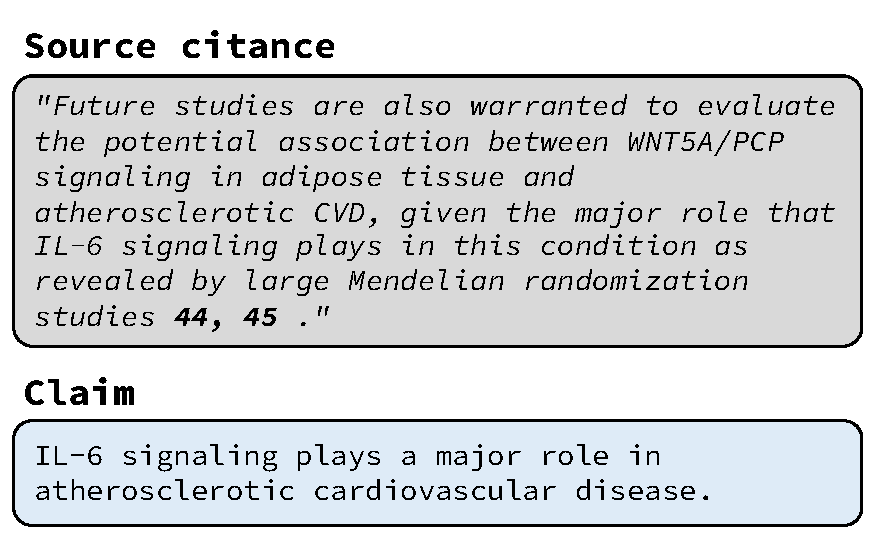
\includegraphics[width=\columnwidth]{figures/claim-fig.pdf}

  \caption{A claim written based on a citance. Material unrelated to the citation is removed. The acronym ``CVD'' is expanded to ``cardiovascular disease''.}
  \label{fig:claim}
\end{figure}

\paragraph{Multiple rationales} Figure \ref{fig:multiple_rationales} shows a claim supported by two rationales from the same abstract. The text of each rationale on its own is sufficient to entail the claim.

\begin{figure}[t]
  \centering

  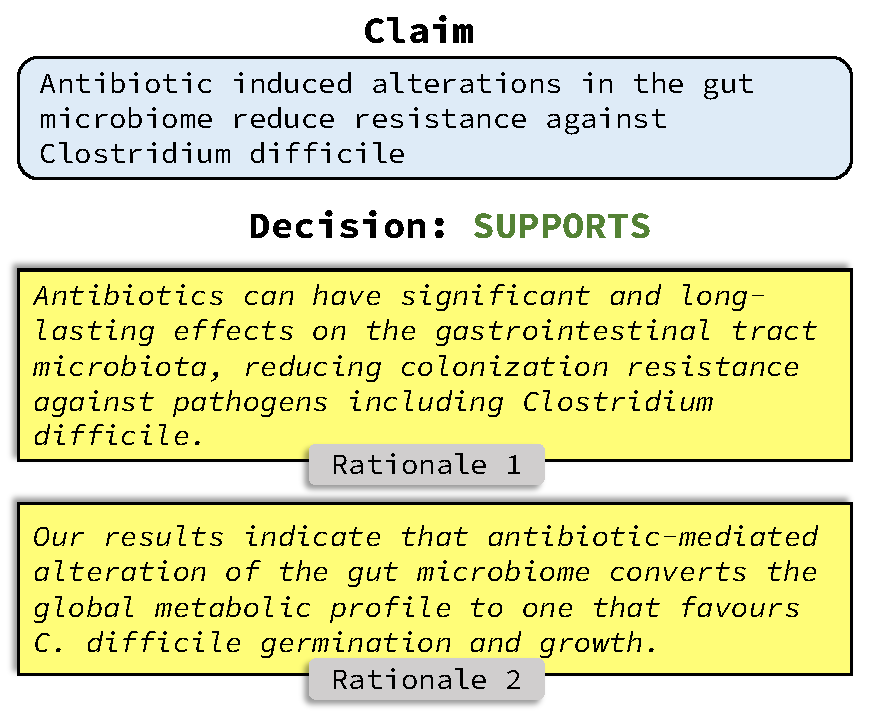
\includegraphics[width=\columnwidth]{figures/multiple-rationales-fig.pdf}
  \caption{A claim supported by two rationales from the same abstract. The text of each rationale on its own provides sufficient evidence to verify the claim.}
  \label{fig:multiple_rationales}

\end{figure}

%%%%%%%%%%%%%%%%%%%%


\subsection{Annotators and quality control}

\paragraph{Claim writing} The claim writers included four experts with background in scientific NLP, fifteen undergraduates studying the life sciences, and four graduate students (doctoral or medical) in the life sciences. Student claim writers attended an in-person training session where they were introduced to the task and received in-person feedback from the four experts. Following training, student annotators continued writing claims remotely. The expert annotators monitored claims for quality during the remote annotation process, and provided feedback when necessary; low-quality claims were returned to the annotators for re-writing. As a final check, all submitted claims were proofread (and edited if necessary) by an undergraduate whose claims were deemed especially high-quality by the expert annotators.

\paragraph{Claim negations}

As mentioned in \S\ref{sec:claim_writing}, an expert annotator wrote claim negations to introduce cases where an abstract \refutes a claim. The annotator skipped claims that could only be negated by adding obvious triggers like ``not''. The majority of claim negations involved a reversal of effect direction; for instance ``\emph{A high microerythrocyte count protects against severe anemia}'' can be negated as ``\emph{A high microerythrocyte count raises vulnerability to severe anemia}''.

\paragraph{Claim verification}

The verifiers included three NLP experts, five undergraduates studying life sciences, and five graduate students studying life sciences. Annotations were performed remotely through a web interface. Annotators were required to pass a 10-question ``quiz'' before annotating their own claims. After passing the quiz, subsequent submissions were reviewed by an NLP expert until that expert deemed the annotator reliable. Approved annotators were then assigned to review each others' submissions. In general, graduate students were assigned to review annotations from undergraduates.


%%%%%%%%%%%%%%%%%%%%


\subsection{Corpus} \label{sec:data_source_appendix}

\paragraph{Additional statistics} Table \ref{tbl:journal_counts} shows the number of cited abstracts from each of our selected journals. The ``Other'' category includes ``co-cited'' (\S\ref{sec:data_source}) abstracts that came from journals not among our pre-defined set.

\begin{table}[t]
  \centering

  \begin{tabular}{l r}
  \toprule
  Journal & Count \\
  \thickmid
  BMJ                            &     60 \\
Blood                          &      8 \\
Cancer Cell                    &      8 \\
Cell                           &     51 \\
Cell Metabolism                &     10 \\
Cell Stem Cell                 &     41 \\
Circulation                    &     12 \\
Immunity                       &     33 \\
JAMA                           &     79 \\
Molecular Cell                 &     27 \\
Molecular Systems Biology      &      5 \\
Nature                         &     29 \\
Nature Cell Biology            &     26 \\
Nature Communications          &     19 \\
Nature Genetics                &      8 \\
Nature Medicine                &     89 \\
Nature Methods                 &      1 \\
Nucleic Acids Research         &     10 \\
Plos Biology                   &     36 \\
Plos Medicine                  &     38 \\
Science                        &      7 \\
Science Translational Medicine &      2 \\
The Lancet                     &     22 \\
\thinmid
Other                          &    120 \\

\thickmid

Total                          &    741 \\
\bottomrule
\end{tabular}

  \caption{Number of cited documents by journal. Some co-cited articles (\S \ref{sec:data_source}) come from journals outside our curated set; these are indicated by ``Other''.}
  \label{tbl:journal_counts}
\end{table}

Figure \ref{fig:mesh_terms} shows counts for the most-frequent MESH terms\footnote{\url{https://www.ncbi.nlm.nih.gov/mesh}} among the cited abstracts. These terms reflect studies ranging from clinical trial reports (``Humans'', ``Middle Aged'', ``Child'') to molecular biology (``Cell Line'', ``RNA'', ``Mutation'').

\begin{figure}[t]
  \centering
  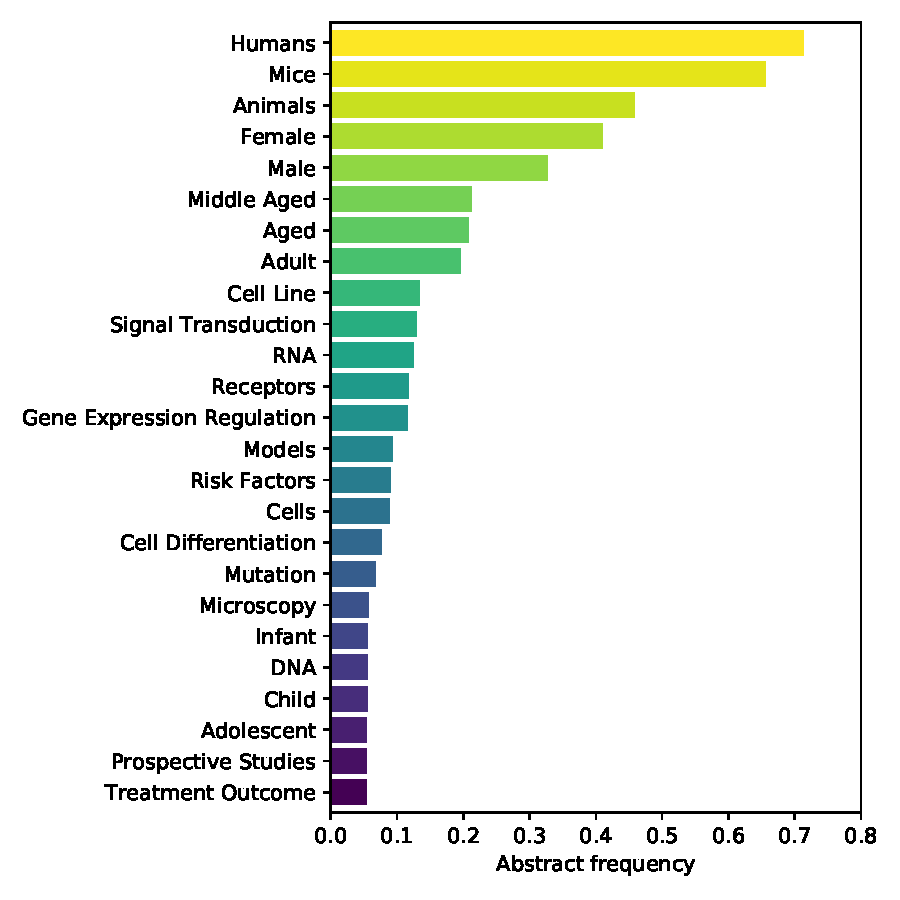
\includegraphics[width=\columnwidth]{figures/mesh-terms-fig.pdf}

  \caption{Fraction of evidence abstracts in which each MESH term occurs.}
  \label{fig:mesh_terms}
\end{figure}

\paragraph{Distractor abstracts} In \S\ref{sec:data_source}, we mention how we increase the size of the corpus by adding \emph{distractor abstracts}. The reason why we do not use the entirety of a large research corpus like S2ORC as our fact-checking corpus is that doing so would introduce many \emph{false negative retrievals}: abstracts containing evidence relevant to a given claim, but not mentioned in the claim's source citance. This can occur either because the citance authors simply were not aware of these abstracts, or because the abstracts were published after the citance was written. These retrievals would be incorrectly marked wrong in by evaluation metrics.

Distractor abstracts as defined in \S\ref{sec:data_source} have two qualities that make them a good addition to the \ours corpus: (1) They are cited in the same articles as our evidence abstracts, meaning that they often discuss similar topics and increase the difficulty of abstract retrieval methods based on lexical similarity. (2) The authors of our citances were aware of the distractor abstracts, and chose not to mention them in the citances used to generate claims. This makes them unlikely to be a source of false positive retrievals.


%%%%%%%%%%%%%%%%%%%%%%%%%%%%%%%%%%%%%%%%%%%%%%%%%%%%%%%%%%%%%%%%%%%%%%%%%%%%%%%%

\section{Annotation interfaces and guidelines} \label{sec:annotation_interfaces}

We show a screenshot of the claim interface in Figure \ref{fig:claim_interface}, and evidence interface in Figure \ref{fig:evidence_interface}.

\begin{figure*}[t]
  \centering
  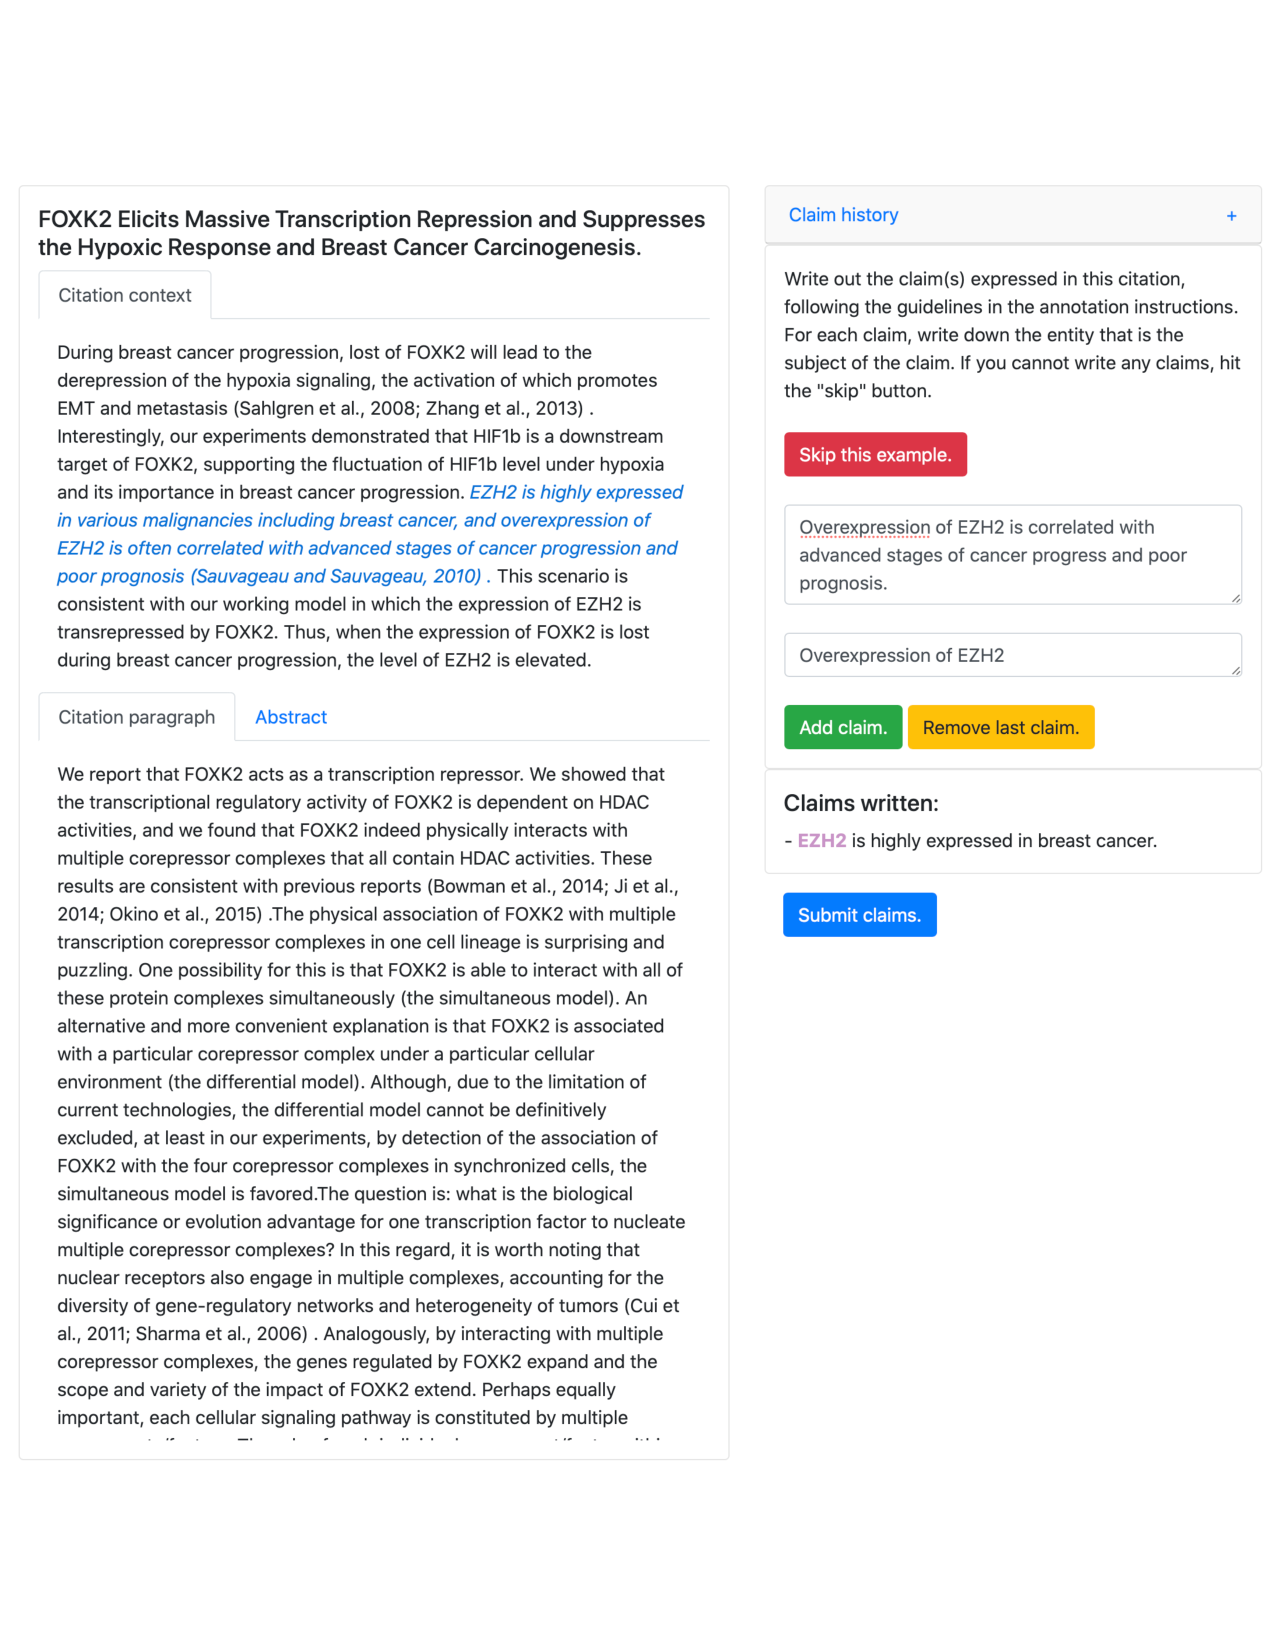
\includegraphics[width=\textwidth]{figures/claim-interface-fig.pdf}

  \caption{The claim-writing interface. The citation sentence is highlighted in blue on the top left. Additional context is provided on bottom left. The right side shows two claims that could be written based on this citation sentence.}
  \label{fig:claim_interface}
\end{figure*}

\begin{figure*}[h]
  \centering
  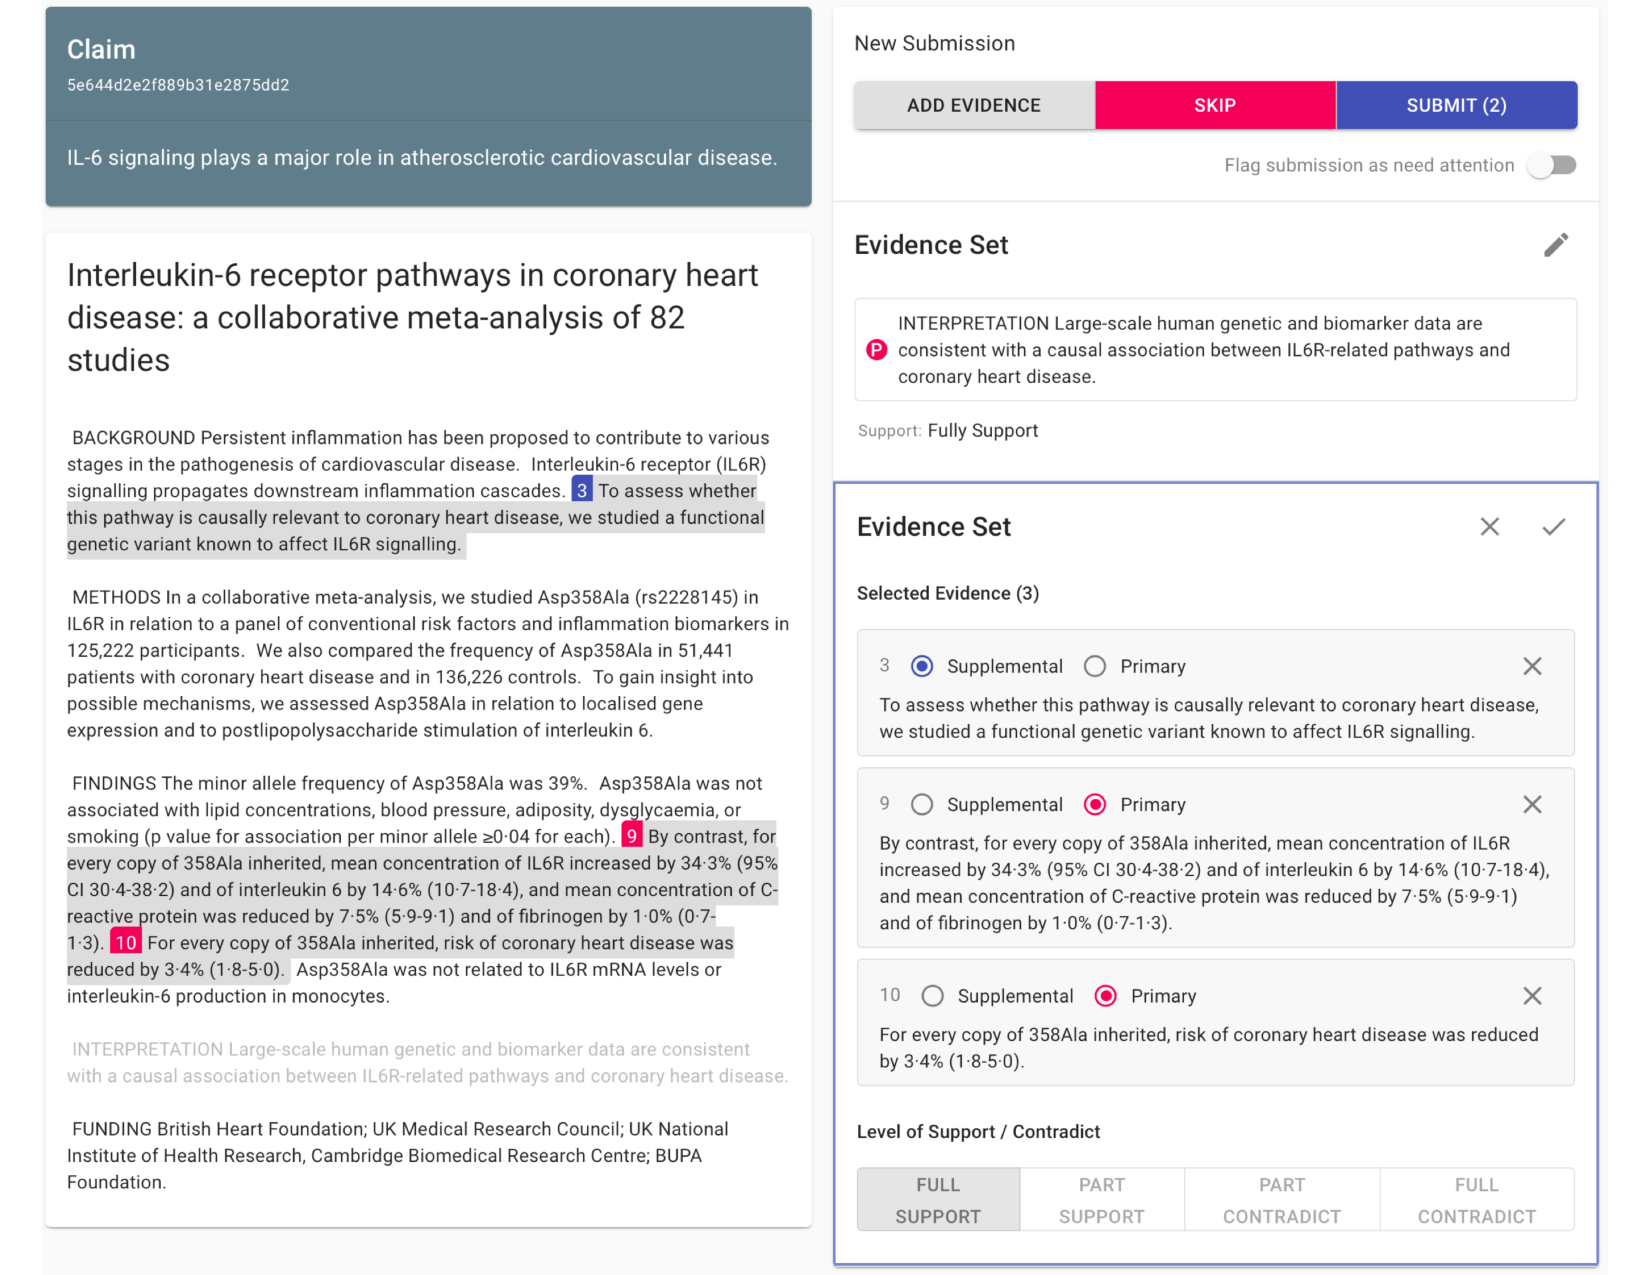
\includegraphics[width=\textwidth]{figures/evidence-interface-fig.pdf}

  \caption{The evidence collection interface.}
  \label{fig:evidence_interface}
\end{figure*}
